\documentclass[tikz]{standalone}
\usepackage{pgfplots}
\usepackage{mathpazo}
\usepackage{amsmath}
\usepgfplotslibrary{polar}
\usepgflibrary{shapes.geometric}
\usetikzlibrary{calc}
\usetikzlibrary{datavisualization}
\usetikzlibrary{datavisualization.formats.functions}
\usetikzlibrary{intersections}
\usetikzlibrary{scopes}
\pgfplotsset{compat=1.12} 
\pgfplotsset{my style/.append style={axis x line=middle, axis y line=middle, xlabel={$x$},ylabel={$y$},smooth}}
\begin{document}
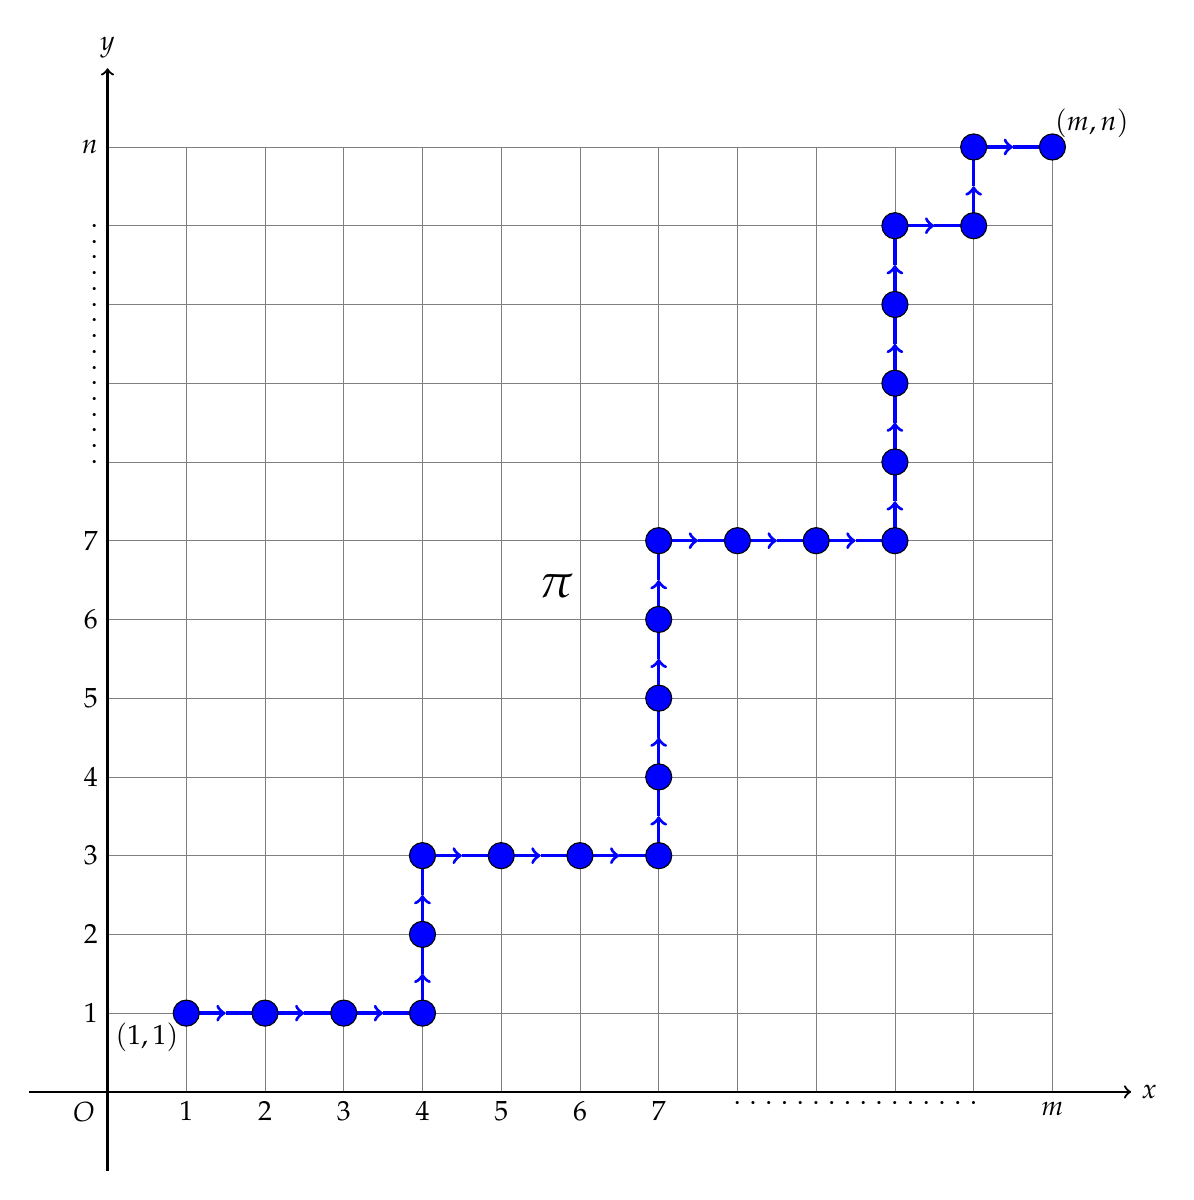
\begin{tikzpicture}[scale=1]
	\draw[gray, very thin] (0, 0) grid (12, 12);
	\draw[->, thick] (-1, 0) -- (13, 0) node[right] {$x$};
	\draw[->, thick] (0, -1) -- (0, 13) node[above] {$y$};
	\foreach \x in {1, 2, 3, 4, 5, 6, 7}
		\draw[xshift = \x cm] node[below] {$\x$};
	\foreach \y in {1, 2, 3, 4, 5, 6, 7}
		\draw[yshift = \y cm] node[left] {$\y$};
	\foreach \x in {8, 8.2, ..., 11}
		\draw[xshift = \x cm] node[below] {$.$};
	\foreach \y in {8, 8.2, ..., 11}
		\draw[yshift = \y cm] node[left] {$.$};
	\foreach \x in {12}
		\draw[xshift = \x cm] node[below] {$m$};
	\foreach \y in {12}
		\draw[yshift = \y cm] node[left] {$n$};
	\draw[->, blue, very thick] (1, 1) -- (1.5, 1);
	\draw[->, blue, very thick] (1.5, 1) -- (2.5, 1);
	\draw[->, blue, very thick] (2.5, 1) -- (3.5, 1);
	\draw[->, blue, very thick] (3.5, 1) -- (4, 1);
	\draw[->, blue, very thick] (4, 1) -- (4, 1.5);
	\draw[->, blue, very thick] (4, 1.5) -- (4, 2.5);
	\draw[->, blue, very thick] (4, 2.5) -- (4, 3);
	\draw[->, blue, very thick] (4, 3) -- (4.5, 3);
	\draw[->, blue, very thick] (4.5, 3) -- (5.5, 3);
	\draw[->, blue, very thick] (5.5, 3) -- (6.5, 3);
	\draw[->, blue, very thick] (6.5, 3) -- (7, 3);
	\draw[->, blue, very thick] (7, 3) -- (7, 3.5);
	\draw[->, blue, very thick] (7, 3.5) -- (7, 4.5);
	\draw[->, blue, very thick] (7, 4.5) -- (7, 5.5);
	\draw[->, blue, very thick] (7, 5.5) -- (7, 6.5);
	\draw[->, blue, very thick] (7, 6.5) -- (7, 7);
	\draw[->, blue, very thick] (7, 7) -- (7.5, 7);
	\draw[->, blue, very thick] (7.5, 7) -- (8.5, 7);
	\draw[->, blue, very thick] (8.5, 7) -- (9.5, 7);
	\draw[->, blue, very thick] (9.5, 7) -- (10, 7);
	\draw[->, blue, very thick] (10, 7) -- (10, 7.5);
	\draw[->, blue, very thick] (10, 7.5) -- (10, 8.5);
	\draw[->, blue, very thick] (10, 8.5) -- (10, 9.5);
	\draw[->, blue, very thick] (10, 9.5) -- (10, 10.5);
	\draw[->, blue, very thick] (10, 10.5) -- (10, 11);
	\draw[->, blue, very thick] (10, 11) -- (10.5, 11);
	\draw[->, blue, very thick] (10.5, 11) -- (11, 11);
	\draw[->, blue, very thick] (11, 11) -- (11, 11.5);
	\draw[->, blue, very thick] (11, 11.5) -- (11, 12);
	\draw[->, blue, very thick] (11, 12) -- (11.5, 12);
	\draw[->, blue, very thick] (11.5, 12) -- (12, 12);
	\draw[circle, draw] (1, 1) node[fill = blue, draw,circle]{}
	      (2, 1) node[fill = blue, draw,circle]{}
	      (3, 1) node[fill = blue, draw]{}
	      (4, 1) node[fill = blue, draw]{}
	      (4, 2) node[fill = blue, draw]{}
	      (4, 3) node[fill = blue, draw]{}
	      (5, 3) node[fill = blue, draw]{}
	      (6, 3) node[fill = blue, draw]{}
	      (7, 3) node[fill = blue, draw]{}
	      (7, 4) node[fill = blue, draw]{}
	      (7, 5) node[fill = blue, draw]{}
	      (7, 6) node[fill = blue, draw]{}
	      (7, 7) node[fill = blue, draw]{}
	      (8, 7) node[fill = blue, draw]{}
	      (9, 7) node[fill = blue, draw]{}
	      (10, 7) node[fill = blue, draw]{}
	      (10, 8) node[fill = blue, draw]{}
	      (10, 9) node[fill = blue, draw]{}
	      (10, 10) node[fill = blue, draw]{}
	      (10, 11) node[fill = blue, draw]{}
	      (11, 11) node[fill = blue, draw]{}
	      (11, 12) node[fill = blue, draw]{}
	      (12, 12) node[fill = blue, draw]{};	
	\draw[xshift = 0.5cm] (12, 12) node[above] {$(m, n)$};
	\draw[xshift = -0.5cm] (1, 1) node[below] {$(1, 1)$};
	\draw[xshift = -0.3cm] (0, 0) node[below] {$O$};
	\draw[xshift = -0.3cm,yshift = -0.3cm]  (6, 7) node[below] {\LARGE$\pi$};
\end{tikzpicture}
\end{document}